\documentclass{article}
\usepackage[utf8]{inputenc}

%additional usepackages
\usepackage{amsmath}
\usepackage{eufrak}
\usepackage{tikz}
\usepackage{ amssymb }
\usepackage{import}
\usepackage[ruled,vlined]{algorithm2e}
\usepackage{booktabs}
\usepackage[capposition=top]{floatrow}
\usepackage{scrextend}
\usepackage{csquotes}
\usepackage{graphicx}
\usepackage{pdfpages}

% bibliography
\usepackage[backend=biber, citestyle=authoryear]{biblatex}
%\addbibresource{acfs.bib}


% margins
\usepackage[margin=1.05in]{geometry}

\newcommand{\E}{\mathbb{E}}
\newcommand{\std}{\mathbf{std}}
\newcommand{\R}{\mathbb{R}}
\newcommand{\G}{\mathcal{G}}
\newcommand{\lra}{\Leftrightarrow}

\newcommand{\la}{\leftarrow}
\newcommand{\ra}{\rightarrow}

\newcommand{\rp}{\right)}
\newcommand{\lp}{\left(}

%%%% INDEPDENT SIGN %%%%

\makeatletter
% Taken from http://ctan.org/pkg/centernot
\newcommand*{\centernot}{%
  \mathpalette\@centernot
}
\def\@centernot#1#2{%
  \mathrel{%
    \rlap{%
      \settowidth\dimen@{$\m@th#1{#2}$}%
      \kern.5\dimen@
      \settowidth\dimen@{$\m@th#1=$}%
      \kern-.5\dimen@
      $\m@th#1\not$%
    }%
    {#2}%
  }%
}
\makeatother

\newcommand{\independent}{\perp\mkern-9.5mu\perp}
\newcommand{\notindependent}{\centernot{\independent}}

%%%%% INDEPENDENT SIGN END %%%%%

\newcommand{\X}{\mathbf{X}}
\newcommand{\Ls}{\mathbf{L}}
\newcommand{\D}{\mathbf{D}}
\newcommand{\W}{\mathbf{W}}

\newcommand{\x}{\mathbf{x}}
\newcommand{\ls}{\mathbf{l}}
\newcommand{\ds}{\mathbf{d}}
\newcommand{\w}{\mathbf{w}}

\newcommand{\rr}{\mathbf{r}}
\newcommand{\RR}{\mathbf{R}}

\newcommand{\ones}{\mathbf{1}}

\DeclareMathOperator*{\argmax}{arg\,max}
\DeclareMathOperator*{\argmin}{arg\,min}


\setlength{\parindent}{0em}
\setlength{\parskip}{0.25cm}

\title{The Effect of Kids on Labour Supply}
\author{Jeppe Søndergaard Johansen (pcv439)}
\date{August 2019}

\makeindex

\begin{document}

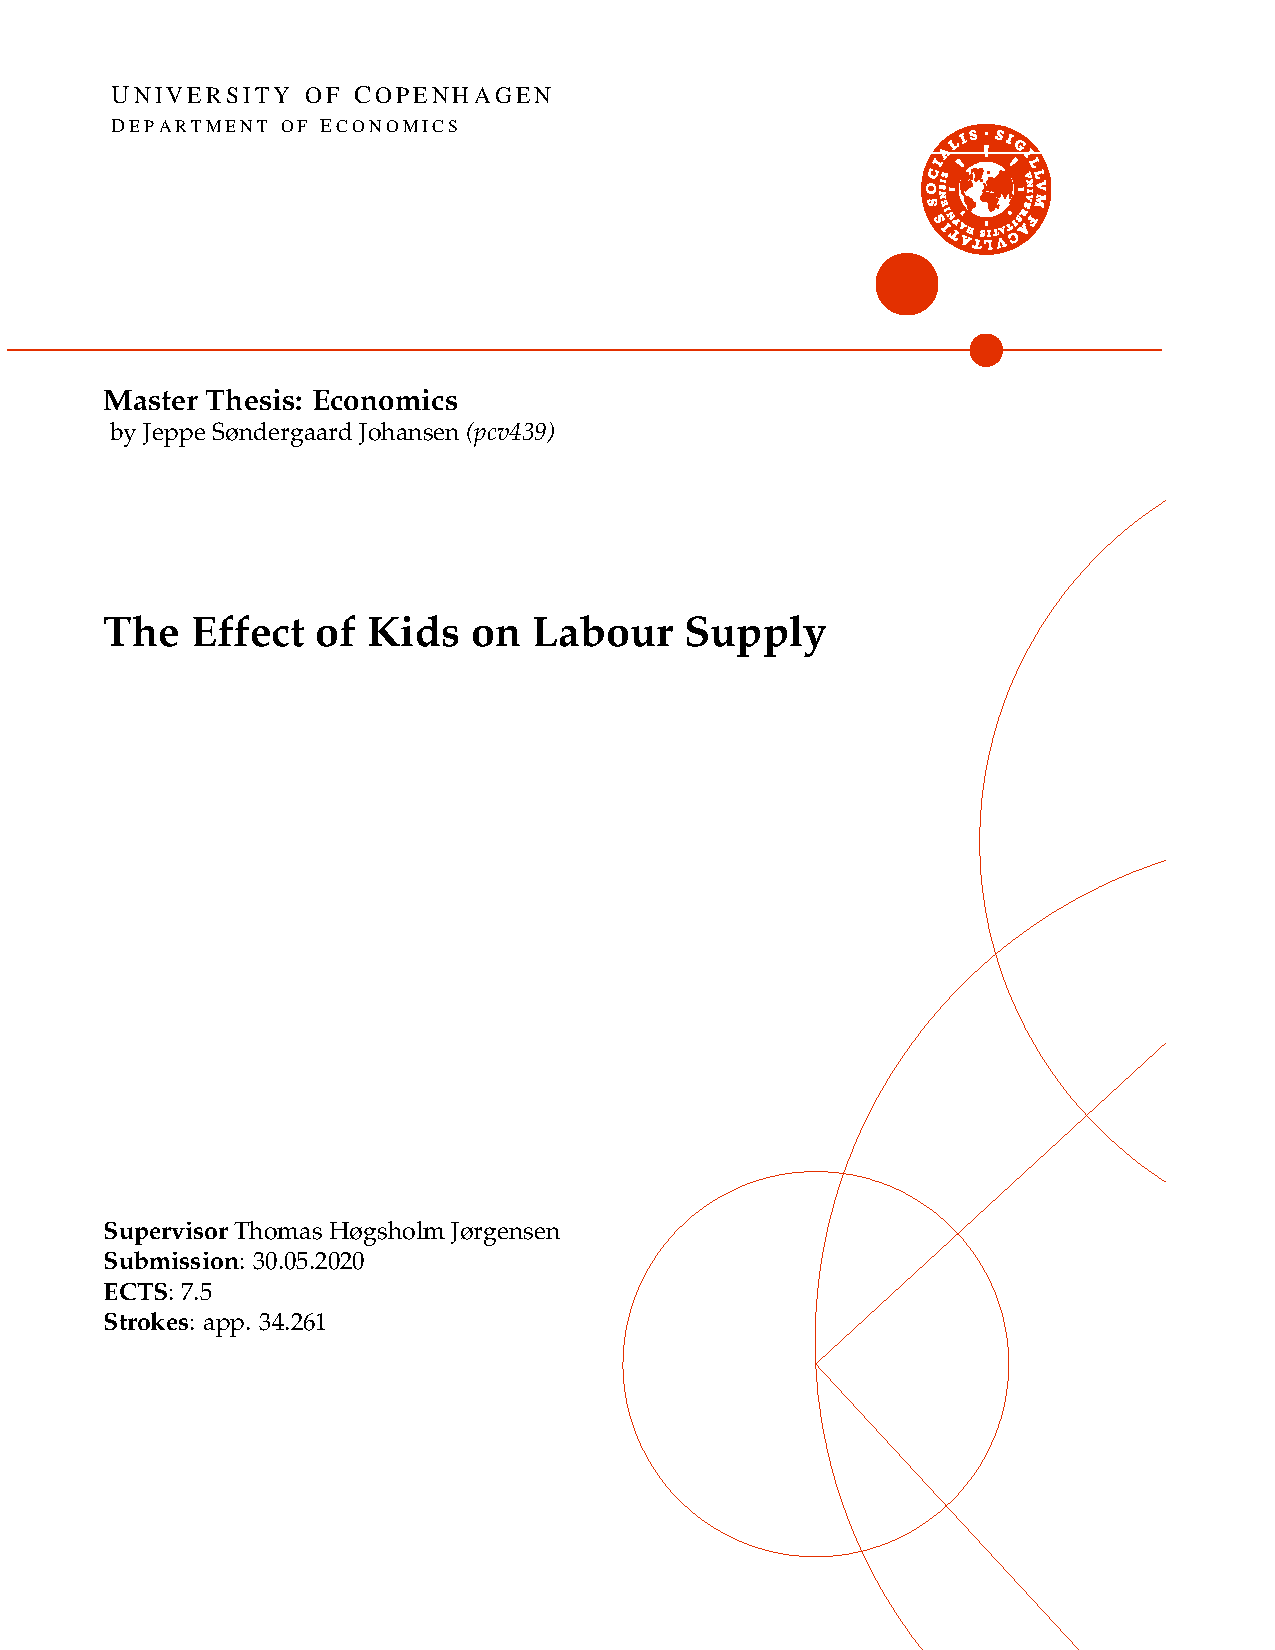
\includepdf[pages={1}]{frontpage/frontpage.pdf}


\maketitle

%\begin{abstract}
This paper investigates reinforcement learning as a solution method for dynamic models. A discrete time, finite horizon, discrete choice model of female labour supply and fertility is formulated, and the model is solved using value function iteration and two reinforcement learning methods, namely deep Q-learning and double deep Q-learning. After estimating the model using method of simulated moments, and finding the simple model inadequate to describe data from Statistic Denmark, the model is extended. The extension consists of 14 + 1 states. The extended model is solved only using double deep Q-learning and estimated using simulated method of moments. The results of the extended model convincingly matches data from Statistics Denmark and contemporary findings by \textcite{kleven_children_2019}. I conclude that the field of economics should further investigate reinforcement learning, as it allows solving dynamic models with high dimensional state space.
\end{abstract}


\pagebreak

\tableofcontents

\pagebreak

\section{Introduction} 

The last 10 years have lead to numerous breakthroughs within the field of machine learning, among them especially the subfield of reinforcement learning has experienced great leaps. In 2013 the company DeepMind achieved super human performance in various Atari games \parencite{mnih_playing_2013}. In 2018 the same company beat professional human players in the board game Go, a feat which was not deemed possible in a foreseeable future \parencite{silver_general_2018}, and as late as 2019 DeepMind showed that an reinforcement learning agent was able to play the game of Star Craft 2 on the same level as the best human players \parencite{vinyals_grandmaster_2019}. All the games mentioned can be considered dynamical models. Dynamic models play a central role within the field of economics. The results imply a new way of solving dynamic economic models using reinforcement learning.

Dynamical models usually involve agents that take sequential actions, trying to maximize the cumulative utility from these actions. This class of economic models conform to a set of properties economists like: They have a micro foundation - agents are utility maximizing. They model time, allowing for agents to foresee the future, and act in accordance to their expectations. Some dynamic models can be solved  analytically. This is true for the canonical Ramsey model. However when the scope of the dynamic model grows, different approaches is necessary. Dynamic programming is usually the tool utilized for solving such models.  Even though dynamic programming is a flexible tool it do have its limitations. Solving a model using dynamic programming, requires a limited sized state space, otherwise the computation involved becomes infeasible. In practice this leaves high dimensional dynamic models impossible to solve using contemporary techniques. Deep reinforcement learning allows for solving such models. Because these techniques are relatively novel, they have not yet been introduced into the field of economics. Deep reinforcement learning, does unfortunately not guarantee that the solution converges to the global maximum, but results have shown that learning is possible in hard, high dimensional environments.

This paper uses the aforementioned techniques to investigate the effect of children on female labour supply. Inspired by the model specification of \textcite{francesconi_joint_2002} and \textcite{adda_career_2011} I formulate an discrete time, finite horizon model that models discreet female labour supply and its relationship to fertility. First a simple model is formulated, where women can choose the number of supplied hours, letting fertility be exogenous, with an income process following the Mincer equation of human capital. The husband of the household, is assumed to follow a deterministic path both with regards to number of hours supplied to the labour force, and with the wage rates they receive. Households are assumed to face a budget constraint, that neither allow for borrowing or saving. Utility is assumed to be a function of leisure and consumption, and children are assumed to reduce leisure by mirroring additional work for the woman, that is not financially compensated. Later an extension to the original model is presented with exogenous education combined with a transfer system for women in the education system. Additionally the extension tracks children on an individual level.

Using three different solution methods: value function iteration, deep Q-learning and double deep Q-learning I solve the simple model. I show that one can get comparable performance using deep reinforcement learning compared to using value function iteration solution methods, yielding a new way to solve more complex dynamic models. The parameters of the Mincer equation are calibrated using data from Statistics Denmark . The model is estimated using method of simulated moments, where a simple grid search approach is applied due to fact the optimization problem being one dimensional. The extended model is only solved using double deep Q-learning. Again the model is estimated using method of simulated moments and grid search. The data used for the optimization is from Statistics Denmark.

My two main findings are: 1) Deep reinforcement learning can yield comparable performance to value function iteration solution methods. Considering this allows for solving dynamic models with high dimensional state space, I argue these methods should be explored further in the field of economics. 2) Simulating from the estimated model, I find the initial simple model is not able fit the data, whereas the extended model does fit the data surprisingly well. Both participation rates and average number of supplied hours to labour force, are surprisingly close to what the data from Statistics Denmark suggest. Comparing to  \textcite{kleven_children_2019}, this paper finds results very similar with regards to earnings, participation rate, supplied hours to the labour force and wage rates, when women gives birth to a child.

The paper follows the structure: A literature review is conducted highlighting the main findings and articles of endogenous female labour supply and the effect of children. A model is formulated based on key takeaways from the literature. The parameters of the income process is calibrated using data from Statistics Denmark. Next, I introduce the reader to both reinforcement learning and deep learning. Settling on three different solution methods i solve and estimate the model. I go on to extend the model, and solve it using double deep Q-Learning. I end by comparing the results to contemporary findings, and data from Statistics Denmark.
\section{Model specification}\label{sec:model1}

This paper presents a discrete time, finite horizon, discrete choice model of female labour supply. More specifically I model a household consisting of wife, husband and a zero or more children. The model attempts to address what the effect of children is on the labour supply of women. The model consists of 3 components: 1) An income and human capital component, 2) A fertility process, 3) A leisure and utility component. I model the households from age $Q_{min}=18$ to the terminal age $Q_{max} = 60$. Here it should be noted, that I make the simplifying assumption that the husband and wife has the same age and that the couple is married from age $Q=18$. The age evolves in a deterministic fashion, i.e. the household grows one year older for each step in the model:

\begin{equation}
    Q_{t+1} = Q_t + 1
\end{equation}

For each time step in the model, the agent has to  choose how many hours the woman of the household should supply on a weekly basis. The choice is discreet, and consists of four action values: $H_t \in \{0, 25, 37, 45 \}$. The labour supply of the man in the households is not a choice variable and is therefore considered an exogenous variable.

The households has two income streams, the husband, which is perfectly deterministic, and the wife. The income process of the wife consists of an idiosyncratic component $Z_t$, which follows a random walk:

\begin{equation}
    Z_{t+1} = Z_t + \epsilon_t, \qquad \epsilon_t \sim \ndist (0, \sigma_\epsilon)
\end{equation}

This allows for agents to do display heterogeneity owing to the fact that some unobserved carrier choices will lead to higher wages, even though two otherwise identical agents have been part of the labour force equally long. Since these job characteristics is unobserved, it is assumed to be a random walk. The second component of the income process is a human capital component based on the Mincer equation, as described by \textcite{lemieux_mincer_2006}. That is the the log-transformed wage rate/wage level can be described by the human capital accumulated:

\begin{equation}
    \log \tilde{W}_t = \alpha + \eta_G G_t + \eta_{G^2} G_t^2
\end{equation}

A couple of things to note. In the original formulation by \textcite{lemieux_mincer_2006}, the education level is also included. However, due to the lack of availability of such data I am not able to condition on this. It should also be noted, that the state $G_t$ represents the human capital accumulated of the woman in the household. Finally this equation governs only the wage rage of the women (not of the husband), for whom the wage rate and the supplied number of hours is considered exogenous. The exogenous wage rate of the husband is found using the data set \textbf{LONS50} from Statistics Denmark. And the number of supplied hours for the husband is found using the data set \textbf{LIGEF15}, again supplied by Statistics Denmark. The wage rate of the women will be capped at the minimum wage if the sum of the two components $\tilde{W}_t + Z_t$ is not above the the minimum wage $W_{min} = 120$: 

\begin{equation}
    W_t = \max ( W_{min}, \tilde{W} + Z_t)
\end{equation}

The human capital accumulation process, follows a formulation allowing for depreciation (or skill atrophy):

\begin{equation}
    G_{t+1} = G_t (1-\delta)  + \frac{1}{37} H_t 
\end{equation}

Where 37 being the standard number of hours worked in Denmark. The total income $Y_t$ of the household can now be formulated as:

\begin{equation}
    Y_t = 46 \cdot W_t \cdot H_t + f^M(Q_t)
\end{equation}

Where $f^M$ represents the income from the husband as a function of age. And $46 \cdot W_t \cdot H_t$ is the number of supplied hours pr. week, $H_t$, times the number of weeks, 46, in a year for the average person on the labour market\footnote{Assuming 6 weeks of holiday.} times the wage rate, $W_t$. The income process is a function of the number of supplied working hours, $H_t$, and the states $(Q_t, Z_t, G_t)$. The parameters $\delta, \sigma_\epsilon, \eta_G, \eta_{G^{2}}$ will be calibrated in section \ref{sec:parameter_calibration}.

The second component of the model is the fertility process. The fertility is assumed to be exogenous depending on the age of the woman. This is summed up in the equation below:

\begin{equation}
    K_{t+1} = K_t+ \psi_t, \qquad \psi_t \mid Q_t \sim Bernoulli (p_\psi(Q_t))
\end{equation}

$K_t$ is the number of children in the household. The household is assumed to start with $K_t = 0$ at age $Q=18$. At each step with probability $p_\psi(Q_t)$ the wife gives birth to a child. Allowing for the accumulation of children. The number of children is capped at a maximum of 5 in the model. The probability $p_\psi(Q_t)$ is modelled using data from Statistics Denmark using the data set \textbf{FOD33}. The number of children $K_t$ is part of the state space. 

The third component of the model is the utility and leisure component. The agent is assumed to get utility from leisure, $L_t$, and consumption, $Y_t$. Following \textcite{francesconi_joint_2002} the households are assumed to face a budget constraint such that all income of period $t$ must be consumed period $t$.The utility $U_t$ is given by:

\begin{equation}
    U_t = \beta_L \ln(L_t + 1) + \beta_Y \ln(Y_t + 1)
\end{equation}

Following the formulation of \textcite{adda_career_2011}, dividing the utility into sub-utility functions, where each sub-utility function allows for curvature by specifying a constant relative risk-averse (CRRA) function for each sub-utility. Assuming the special case of $\ln(\cdot)$. The parameters $\beta_L, \beta_Y$ is the individual weighing of the different sub-utilities. Note that for identification I will restrict $\beta_Y= 1$. The total number of hours leisure the agent receives in a year follows: 

\begin{equation}
    L_t = 46 \lp \lp 24 \cdot 7 \rp - \omega \cdot K_t - H_t \rp
\end{equation}

Following \textcite{firestone_estimation_1988}, \textcite{thrane_men_2000} and \textcite{ekert-jaffe_time_2015} I assume that some of the time spent with children can be considered work. The number of hours spent on children each week is captured by $-\omega \cdot K_t$. I let $\omega=3.5$ be the time spent of extra house work pr. child each week. This number is taken from \textcite{ekert-jaffe_time_2015}. The weekly number of hours supplied to the labour market $H_t$ is also subtracted from the total amount of leisure. The number of hours is aggregated to annual level subtracting 6 weeks for holiday. To conclude $\beta_L$ will be a parameter estimated to give the best fit of the model

Summarizing the model; the model contains 4 states: $(G)$ human capital, $(Z)$ the idiosyncratic wage path, $(K)$ the number of children in the household and lastly $(Q)$ age. The action taken in each period $(H)$ represents the number of hours the woman supplies to the labour market on a weekly basis. Other important variables are: $(W)$ the wage rate, $(\tilde{W})$ the human capital dependent wage rate,  $(U)$ the utility and $(L)$ leisure. Formally this imply:

\begin{equation}
    \textbf{State space: }\statespace = \R^{2} \times \{0, 1, 2, 3, 4, 5\} \times \{ 18, 19, \cdots, 60\}
\end{equation}

\begin{equation}
    \textbf{Action space: }\actionspace  = \{0, 15, 25, 37, 45\} 
\end{equation}

\begin{equation}
    \textbf{States: }\{G, Z, K, Q\}, \qquad \textbf{Actions: } \{H\} 
\end{equation}

The model furthermore contains the following parameters: $\alpha, \eta_G, \eta_{G^2}, \delta, \sigma_\epsilon, \beta_L, \beta_Y=1, W_{min}=120, \omega=3.5$. Where the parameters governing the income process $(\alpha, \eta_G, \eta_{G^2}, \delta, \sigma_\epsilon)$ will be calibrated using a simple agent based model, and $\beta_L$ will be estimated using the full model. The recursive formulation of the model is given below:

\begin{align}
    U_t(L_t, Y_t) &= \beta_L \ln(L_t + 1) + \beta_Y \ln(Y_t + 1) \label{eq:utility_v1}\\
    L_t(K_t, H_t) &= 46 \cdot ((24 \cdot 7) - \omega \cdot K_t  - H_t) \label{eq:leissure_v1}\\
    \log \tilde{W}_t (G_t) &= \alpha + \eta_G G_t + \eta_{G^2} G_t^2 \label{eq:salary_tilde_v1}\\
    W_t(\tilde{W}_t, Z_t) &= \max(W_{min} , \tilde{W}_t  + Z_t)  \label{eq:salary_v1}\\
    Y_t(Q_t,H_t, W_t) &= 46 \cdot H_t \cdot W_t + f^M(Q_t) \label{eq:total_salary_v1}\\
\end{align}

Law of motion:

\begin{align}
    Q_{t+1}(Q_t) &= Q_t \label{eq:age_v1}\\
    K_{t+1}(K_t, Q_t)  &= K_{t} + \psi_t, \qquad \psi_t \mid Q_t \sim Bernoulli(p_\psi(Q_t)) \label{eq:fertility_v1} \\
    Z_{t+1}(Z_t) &= Z_t + \epsilon_t, \qquad \epsilon_t \sim \ndist(0, \sigma_\epsilon) \label{eq:idiosyncratic_wage_path_v1}\\
    G_{t+1}(G_t) &= G_t(1 - \delta) + \frac{1}{37} H_t \\
\end{align}



\section{Model (Extended)}

This will be where the extended model will be.

\end{document}
